%Iniciação de pacotes e linguagens
\documentclass[12pt]{article}
\usepackage{fatec-ti}
\usepackage{url}
\def\UrlBreaks{\do\/\do-}
\usepackage{graphicx,url}
\usepackage[brazil]{babel}   
\usepackage[utf8]{inputenc}
\usepackage{longtable}
\usepackage{tabularx}
\usepackage{float}
\sloppy

% Título do TCC - Projeto Integrador - Trabalho
% As contra barras são para inserir uma segunda linha ao título
\title{JangoPRO\\Faculdade de Tecnologia SENAC Pelotas}

% Nome do Autor e do Orientador
    \author{Pedro Couto Campos\inst{1}, Angelo Luz\inst{1}}

% Endereço da Faculdade
\address{Curso de ADS -- Faculdade de Tecnologia SENAC Pelotas\\
  Rua Gonçalves Chaves 602 -- 96015560 -- Pelotas -- RS -- Brazil
  \email{pedrocoutocampos@outlook.com}
}

\begin{document} 

\maketitle

% Resumo em inglês - ABSTRACT (não devendo ultrapassar 10 linhas)
\begin{abstract}
  The proposed system aims to facilitate the administration of a barbershop, streamlining services scheduling, payment processing, and overall company workflow control. This system targets small to medium-sized barbershops, providing a comprehensive solution to enhance both owners' and clients' experiences.

  \textbf{Keywords}: barbershop management, scheduling, payment processing, workflow control, small business.
\end{abstract}

\begin{resumo} 
  O sistema proposto tem como objetivo facilitar a administração de uma barbearia, simplificando o agendamento de serviços, processamento de pagamentos e controle geral do fluxo da empresa. Este sistema destina-se a barbearias de pequeno e médio porte, fornecendo uma solução abrangente para aprimorar as experiências tanto dos proprietários quanto dos clientes.

  \textbf{Palavras-Chave}: gestão de barbearia, agendamento, processamento de pagamentos, controle de fluxo, pequenos negócios.
\end{resumo}


%Seções...
% As seções quando criadas, automaticamente seguem uma sequência numérica, mesmo caso para as sub-seções
\section{Introdução} 


\paragraph{}No contexto contemporâneo, a eficiência na administração de negócios tornou-se um elemento crucial para o sucesso empresarial. Compreender e atender às demandas específicas de uma empresa é essencial para a otimização de processos e a maximização de resultados. Este trabalho tem como propósito apresentar e desenvolver um sistema dedicado à gestão abrangente de uma barbearia, atendendo às necessidades específicas do proprietário e visando aprimorar a eficiência operacional.


A gestão eficaz de uma barbearia envolve uma série de desafios, desde o controle financeiro até a administração de recursos humanos. Este sistema proposto visa ser uma ferramenta integrada que não apenas simplifica, mas aprimora a administração do estabelecimento. Dentre os principais objetivos, destacamos a facilitação do controle financeiro, permitindo um monitoramento preciso das receitas e despesas, bem como o gerenciamento eficiente do quadro de pessoal.


Um dos principais diferenciais deste sistema reside na agilidade proporcionada ao serviço de agendamento e atendimento. Reconhecendo a importância do tempo no contexto moderno, a proposta é reduzir significativamente a espera dos clientes, garantindo uma experiência mais eficiente e satisfatória. A rapidez na execução dos serviços não apenas aumenta a satisfação do cliente, mas também contribui para a otimização do fluxo de trabalho interno.


Ao longo deste artigo, serão abordadas as funcionalidades específicas do sistema, bem como a sua arquitetura e as tecnologias empregadas. Além disso, será discutido o embasamento teórico que sustenta a importância da implementação de sistemas de gestão em estabelecimentos desse segmento.


Em suma, o desenvolvimento deste sistema de gestão para barbearias visa não apenas atender, mas exceder as expectativas do proprietário, proporcionando uma ferramenta robusta e eficiente para aprimorar a administração do negócio e elevar a qualidade dos serviços prestados. Este trabalho busca contribuir para o avanço no campo da gestão de negócios no setor de barbearias, alinhando-se às demandas contemporâneas e promovendo uma visão inovadora para a eficiência operacional.


\section{Referencial Teórico}

O referencial teórico desta pesquisa visa oferecer uma base sólida para a compreensão das tecnologias, práticas e tendências que norteiam o desenvolvimento de sistemas para gestão de barbearias. Ao explorar esse campo, é possível identificar elementos essenciais que contribuem para a eficiência e competitividade do sistema proposto.

\subsection{Tecnologias Emergentes em Gestão Empresarial}

No âmbito da gestão empresarial, a incorporação de tecnologias emergentes desempenha um papel crucial na otimização de processos. Sistemas de informação integrados, baseados em nuvem, têm se destacado, proporcionando flexibilidade, acessibilidade remota e segurança na gestão de dados. A utilização dessas tecnologias não só simplifica a administração, mas também viabiliza a coleta e análise de dados estratégicos para tomada de decisões embasadas.

\subsection{Sistemas de Agendamento e Atendimento}

A eficácia de um sistema de barbearia está intrinsecamente ligada à capacidade de agendamento e gerenciamento de atendimentos. A implementação de um sistema de agendamento online não apenas facilita a vida do cliente, mas também otimiza o tempo de trabalho dos profissionais. Tecnologias de notificação automática e lembretes são ferramentas que contribuem para a redução de faltas e atrasos, garantindo um fluxo mais organizado e eficiente.

\subsection{Controle Financeiro e Contábil}

A gestão financeira é um aspecto vital para o sucesso sustentável de qualquer empreendimento. Sistemas que integram controles financeiros e contábeis oferecem uma visão abrangente das receitas, despesas e lucratividade. A automação de processos contábeis não apenas reduz erros, mas também agiliza a geração de relatórios e demonstrativos, fornecendo ao gestor informações cruciais para a tomada de decisões estratégicas.

\subsection{Tendências em Experiência do Cliente}

A experiência do cliente é um diferencial competitivo significativo. Sistemas que incorporam elementos de personalização, feedback automatizado e programas de fidelidade contribuem para a construção de relacionamentos sólidos. A integração de tecnologias que visam aprimorar a experiência do cliente não se resume apenas ao momento do atendimento, mas também abrange estratégias pós-serviço, visando a fidelização e recomendação.

\subsection{Segurança de Dados e Privacidade}

Em um cenário onde a segurança da informação é primordial, sistemas de gestão devem adotar práticas e tecnologias que garantam a integridade e confidencialidade dos dados. A conformidade com regulamentações de proteção de dados, como o GDPR, e a implementação de protocolos de segurança robustos são aspectos críticos para a confiança do cliente e a reputação do negócio.

Em resumo, o referencial teórico apresentado destaca a importância de abraçar as tendências tecnológicas emergentes, incorporando práticas eficientes e inovadoras na concepção de sistemas de gestão para barbearias. Esses elementos são fundamentais para assegurar a competitividade do negócio, proporcionando uma administração eficiente e uma experiência positiva para clientes e colaboradores.

\subsection{Trabalhos Relacionados}

Dois sistemas amplamente reconhecidos no contexto de gestão para salões de beleza e barbearias são Booksy e Beauty Date. Ambos desempenham papéis significativos na facilitação da administração e na melhoria da experiência tanto para os proprietários quanto para os clientes.

\subsection{Booksy}

Booksy é uma plataforma abrangente projetada para atender às necessidades específicas de estabelecimentos de beleza, incluindo salões de cabeleireiro e barbearias. Sua funcionalidade principal reside no agendamento online, permitindo que os clientes marquem horários de maneira conveniente. Além disso, o Booksy oferece recursos para gestão de clientes, controle financeiro e acompanhamento de desempenho dos profissionais.

Uma característica distintiva do Booksy é a sua interface intuitiva, tanto para os clientes quanto para os profissionais. Isso contribui para uma experiência de agendamento simplificada, aumentando a eficiência do processo. A plataforma também incorpora recursos de notificação automatizada, ajudando a reduzir no-shows e garantindo uma operação mais fluida.

\subsection{Beauty Date}

O Beauty Date é outra solução abrangente voltada para a gestão de salões de beleza e barbearias. Semelhante ao Booksy, destaca-se pela sua capacidade de agendamento online, permitindo que os clientes escolham horários disponíveis de forma conveniente. Além do agendamento, o Beauty Date oferece funcionalidades como controle financeiro, gestão de estoque e acompanhamento do desempenho dos profissionais.


Uma característica distintiva do Beauty Date é a ênfase na personalização e fidelização do cliente. O sistema permite a criação de programas de pontos e ofertas personalizadas, incentivando a retenção de clientes e promovendo a satisfação. Isso alinha-se às tendências contemporâneas, onde a experiência do cliente desempenha um papel central na competitividade do negócio.

Ambos os sistemas, Booksy e Beauty Date, ilustram a importância de soluções tecnológicas dedicadas à gestão eficiente de barbearias. Suas funcionalidades abrangentes e foco na experiência do cliente destacam a relevância de incorporar tais elementos no desenvolvimento do sistema proposto neste trabalho. A análise dessas plataformas serve como um guia valioso para a implementação de funcionalidades eficazes e inovadoras em nosso sistema de gestão para barbearias.

\section{Projeto de Sistema}

O sistema proposto visa atender às necessidades específicas de barbearias de médio e pequeno porte, proporcionando uma solução abrangente para facilitar o dia a dia da administração e melhorar a experiência tanto dos proprietários quanto dos clientes.

\subsection{Levantamento de Requisitos}

\subsubsection{Requisitos Funcionais}

\begin{itemize}
    \item \textbf{[RF001] Realizar o cadastro da Barbearia:}
    \begin{itemize}
        \item \textbf{Descrição:} Permitir o cadastro da barbearia com autenticação por nome, e-mail e senha.
        \item \textbf{Critérios de Aceitação:}
        \begin{itemize}
            \item A autenticação deve ocorrer por nome da barbearia, e-mail e senha.
        \end{itemize}
    \end{itemize}
    \item \textbf{[RF002] Realizar o agendamento do cliente:}
    \begin{itemize}
        \item \textbf{Descrição:} Possibilitar o agendamento de clientes com informações como nome, data e hora.
        \item \textbf{Critérios de Aceitação:}
        \begin{itemize}
            \item O agendamento deve conter nome, data e hora.
        \end{itemize}
    \end{itemize}
    \item \textbf{[RF003] Escolher o tipo do corte do cliente:}
    \begin{itemize}
        \item \textbf{Descrição:} Permitir que o cliente escolha o tipo de corte desejado.
        \item \textbf{Critérios de Aceitação:}
        \begin{itemize}
            \item O sistema deve registrar o tipo de corte selecionado pelo cliente.
        \end{itemize}
    \end{itemize}
    \item \textbf{[RF004] Controle de agendamentos:}
    \begin{itemize}
        \item \textbf{Descrição:} Manter um controle dos agendamentos do dia.
        \item \textbf{Critérios de Aceitação:}
        \begin{itemize}
            \item O sistema deve exibir os agendamentos do dia para os barbeiros e administradores.
        \end{itemize}
    \end{itemize}
    \item \textbf{[RF005] Login através de e-mail e senha:}
    \begin{itemize}
        \item \textbf{Descrição:} Autenticação por meio de e-mail e senha, com senha contendo pelo menos 8 dígitos.
        \item \textbf{Critérios de Aceitação:}
        \begin{itemize}
            \item A autenticação deve ocorrer por e-mail e senha.
            \item A senha fornecida deve ter no mínimo 8 dígitos.
        \end{itemize}
    \end{itemize}
    \item \textbf{[RF006] Cadastrar cortes:}
    \begin{itemize}
        \item \textbf{Descrição:} Possibilitar o cadastro dos diferentes cortes oferecidos pela barbearia.
        \item \textbf{Critérios de Aceitação:}
        \begin{itemize}
            \item Os barbeiros e administradores devem poder cadastrar os tipos de cortes disponíveis.
        \end{itemize}
    \end{itemize}
    \item \textbf{[RF007] Escolher o tipo do plano:}
    \begin{itemize}
        \item \textbf{Descrição:} Permitir que o cliente escolha entre planos básico ou premium.
        \item \textbf{Critérios de Aceitação:}
        \begin{itemize}
            \item O sistema deve oferecer opções de planos (básico ou premium) para os clientes escolherem.
        \end{itemize}
    \end{itemize}
    \item \textbf{[RNF008] Realizar o cadastro do Barbeiro:}
    \begin{itemize}
        \item \textbf{Descrição:} Permitir o cadastro de novos barbeiros com informações como nome, telefone e e-mail.
        \item \textbf{Critérios de Aceitação:}
        \begin{itemize}
            \item O sistema deve fornecer uma interface de cadastro para os administradores inserirem os dados do barbeiro.
            \item Os campos de nome, telefone e e-mail devem ser obrigatórios.
            \item O campo de e-mail deve conter um endereço de e-mail válido.
            \item O campo de telefone deve aceitar apenas números, podendo conter caracteres especiais para formatação.
        \end{itemize}
    \end{itemize}
    \item \textbf{[RNF009] Login do cliente:}
    \begin{itemize}
        \item \textbf{Descrição:} Permitir que os clientes façam login utilizando seu endereço de e-mail e senha.
        \item \textbf{Critérios de Aceitação:}
        \begin{itemize}
            \item O sistema deve fornecer uma interface de login para que os usuários insiram seu e-mail e senha.
            \item Tanto o e-mail quanto a senha são obrigatórios para o login.
            \item O sistema deve validar se o e-mail contém um endereço de e-mail válido.
            \item A senha fornecida pelo usuário deve conter pelo menos 8 caracteres.
        \end{itemize}
    \end{itemize}
    \item \textbf{[RNF010] Agendamento de Horário pelo Cliente:}
    \begin{itemize}
        \item \textbf{Descrição:} Permitir que os clientes autenticados entrem no sistema e agendem um horário na barbearia de acordo com a disponibilidade.
        \item \textbf{Critérios de Aceitação:}
        \begin{itemize}
            \item Apenas usuários autenticados podem acessar a funcionalidade de agendamento.
            \item O sistema deve fornecer uma interface de agendamento clara e intuitiva.
            \item Os usuários devem poder selecionar a data e o horário desejados para o agendamento.
            \item O sistema deve mostrar apenas os horários disponíveis para agendamento.
        \end{itemize}
    \end{itemize}
\end{itemize}

\subsection{Requisitos Não Funcionais}

\begin{itemize}

   \item \textbf{[RNF001] Senhas serão criptografadas:}
    \begin{itemize}
        \item As senhas dos usuários serão armazenadas de forma segura, utilizando algoritmos de criptografia.
    \end{itemize}
    \item \textbf{[RNF002] Menus e telas intuitivas:}
    \begin{itemize}
        \item A interface do sistema será projetada de forma intuitiva, facilitando a navegação e utilização pelos usuários.
    \end{itemize}
    \item \textbf{[RNF003] Frameworks serão NestJS, GRAPHQL e TYPEORM:}
    \begin{itemize}
        \item O sistema será desenvolvido utilizando os frameworks NestJS para o backend, GRAPHQL para a comunicação entre cliente e servidor, e TYPEORM para a manipulação do banco de dados.
    \end{itemize}
    \item \textbf{[RNF004] Frameworks serão React, NextJS:}
    \begin{itemize}
        \item O frontend do sistema será desenvolvido utilizando os frameworks React e NextJS.
    \end{itemize}
    \item \textbf{[RNF005] Front-End e Back-End serão em TypeScript:}
    \begin{itemize}
        \item Tanto o frontend quanto o backend serão desenvolvidos em TypeScript, proporcionando um código mais robusto e fácil de manter.
    \end{itemize}
    \item \textbf{[RNF006] Banco de dados será PostgreSQL:}
    \begin{itemize}
        \item O sistema utilizará o banco de dados PostgreSQL para armazenar de forma segura e eficiente as informações necessárias.
    \end{itemize}
    \item \textbf{[RNF007] Ambiente será Dockerizado:}
    \begin{itemize}
        \item O ambiente de desenvolvimento e produção será dockerizado, facilitando a replicação e distribuição do sistema.
    \end{itemize}
\end{itemize}

Este levantamento de requisitos forma a base para o desenvolvimento do sistema de barbearia, garantindo que as funcionalidades essenciais sejam atendidas e que aspectos não funcionais como segurança, usabilidade e tecnologias escolhidas sejam considerados.

\subsection{Casos de Uso}

Apresentar e comentar o diagrama de casos de uso da aplicação
\begin{figure}[h]
\centering
    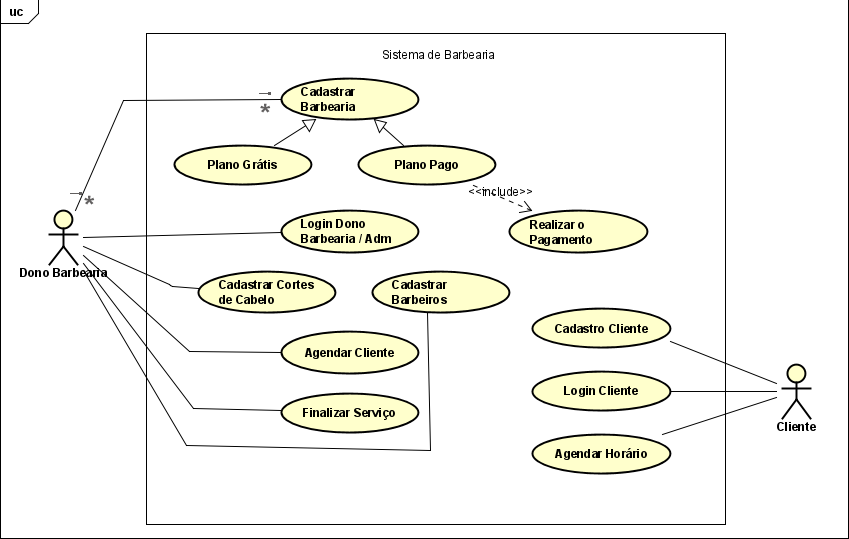
\includegraphics[width=.3\textwidth]{imgs/Diagrama Casos de Uso JangoPRO.png}
    \caption{Diagrama de Casos de Uso do JangoPRO}
    \label{fig:casos-de-uso}
\end{figure}

\subsection{Diagrama Entididade Relacionamento}

Apresentar e comentar o diagrama ER da aplicação.

\begin{figure}[ht]
\centering
    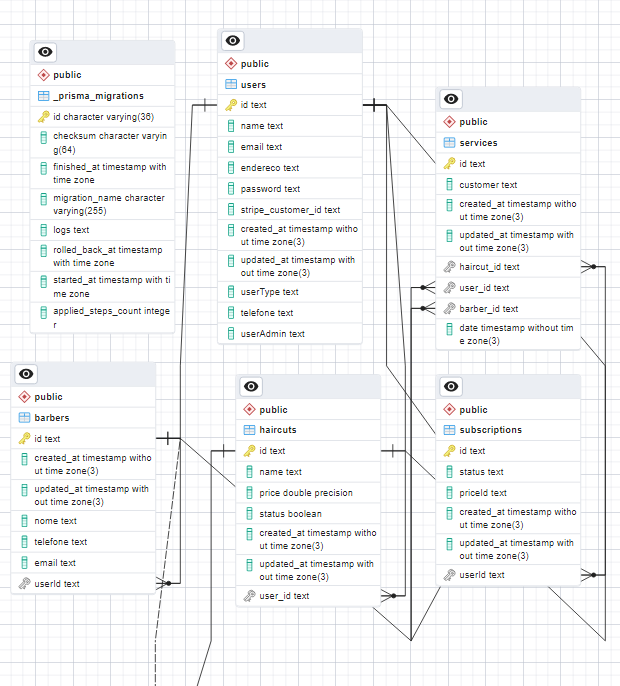
\includegraphics[width=.3\textwidth]{imgs/Diagrama de Classes JangoPRO.png}
    \caption{Diagrama de Classes do JangoPRO}
    \label{fig:casos-de-classes}
\end{figure}

\section{Tecnologias do Projeto}

\subsection{API}

\begin{itemize}
    \item \textbf{Prisma:} Prisma é um moderno ORM (Object-Relational Mapping) para Node.js e TypeScript, simplificando a interação com o banco de dados PostgreSQL.
    
    \item \textbf{Node.js:} Node.js é um ambiente de execução JavaScript do lado do servidor, permitindo o desenvolvimento de aplicativos escaláveis e de alta performance.
    
    \item \textbf{PostgreSQL:} PostgreSQL é um sistema de gerenciamento de banco de dados relacional, conhecido por sua confiabilidade e suporte a transações complexas.
    
    \item \textbf{TypeScript:} TypeScript, uma linguagem superset do JavaScript, adiciona tipagem estática ao código, melhorando a robustez e identificação precoce de erros.
\end{itemize}

\begin{itemize}
    \item \textbf{Next.js:} Next.js é um framework React que simplifica o desenvolvimento de aplicações, oferecendo recursos como renderização do lado do servidor e geração de páginas estáticas.
    
    \item \textbf{React:} React, uma biblioteca JavaScript para construção de interfaces de usuário, permite a criação de componentes reutilizáveis e interfaces dinâmicas.
    
    \item \textbf{TypeScript (no Frontend):} A utilização de TypeScript no frontend proporciona benefícios adicionais de tipagem estática ao JavaScript, garantindo consistência no código.
\end{itemize}

\begin{figure}[ht]
    \centering
    
\includegraphics[width=.3\textwidth]{imgs/Linguagens e Tec do Projeto.png}
    \caption{Arquitetura}
    \label{fig:arquitetura}
\end{figure}

Essa escolha de tecnologias forma uma pilha robusta e escalável para o desenvolvimento de aplicações web modernas. A consistência do código é aprimorada pelo uso de TypeScript em ambos os lados, e o Next.js traz benefícios significativos, como otimizações de performance e simplificação na implementação de rotas e páginas.

\section{JangoPRO}

Ao analisar os requisitos funcionais do JangoPRO em comparação com os sistemas relacionados previamente apresentados, destacam-se características distintivas que posicionam o JangoPRO como uma solução inovadora e abrangente para a gestão de barbearias de médio e pequeno porte.

\subsection{Diferenciais Baseados nos Requisitos Funcionais:}

\paragraph{} 1. \textbf{Cadastro e Autenticação Simplificados:}
   - O JangoPRO simplifica o processo de cadastro da barbearia, adotando autenticação por nome, e-mail e senha. Essa abordagem proporciona facilidade de acesso, garantindo que os estabelecimentos possam rapidamente integrar-se ao sistema.

2. \textbf{Agendamento Personalizado:}
   - A capacidade de escolher o tipo de corte desejado e a opção de agendamento com nome, data e hora oferecem uma experiência de agendamento personalizada para os clientes. Isso contribui para a fidelização, permitindo que os clientes expressem suas preferências individuais.

3. \textbf{Controle de Agendamentos Eficiente:}
   - O controle de agendamentos do JangoPRO vai além do básico, proporcionando uma visão detalhada dos agendamentos do dia. Isso não apenas otimiza a gestão do tempo para os profissionais, mas também minimiza as demoras nos serviços.

4. \textbf{Cadastro de Cortes e Planos:}
   - A funcionalidade de cadastrar diferentes tipos de cortes e escolher entre planos básico ou premium destaca a flexibilidade do JangoPRO. Essa personalização não apenas atende às particularidades de cada barbearia, mas também reflete uma compreensão da diversidade de serviços oferecidos.

5. \textbf{Cadastro de Barbeiros com Informações Essenciais:}
   - A inclusão do requisito de cadastro de barbeiros, com informações como nome, telefone e e-mail, visa não apenas à inclusão de profissionais, mas também à criação de uma base de dados detalhada para melhor administração.

6. \textbf{Login de Clientes e Agendamento Online:}
   - A funcionalidade de login para clientes, com autenticação por e-mail e senha, facilita o acesso ao sistema. O agendamento online, condicionado à autenticação, reforça a praticidade para os clientes e a eficiência para os estabelecimentos.

Ao reunir esses diferenciais, o JangoPRO se posiciona como uma solução abrangente e eficiente para a gestão de barbearias, integrando as funcionalidades necessárias para atender tanto às demandas operacionais quanto às expectativas dos clientes.

Em seguida, principais telas do sistema e suas funcionalidades.
\begin{figure}[!ht]
    \centering
    
\includegraphics[width=.3\textwidth]{imgs/Tela Login.png}
    \caption{Tela Login}
    \label{fig:login}
\end{figure}
\begin{figure}[!ht]
    \centering
    
\includegraphics[width=.3\textwidth]{imgs/Tela Cadastrar.png}
    \caption{Cadastrar}
    \label{fig:cadastrar}
\end{figure}
\begin{figure}[!ht]
    \centering
    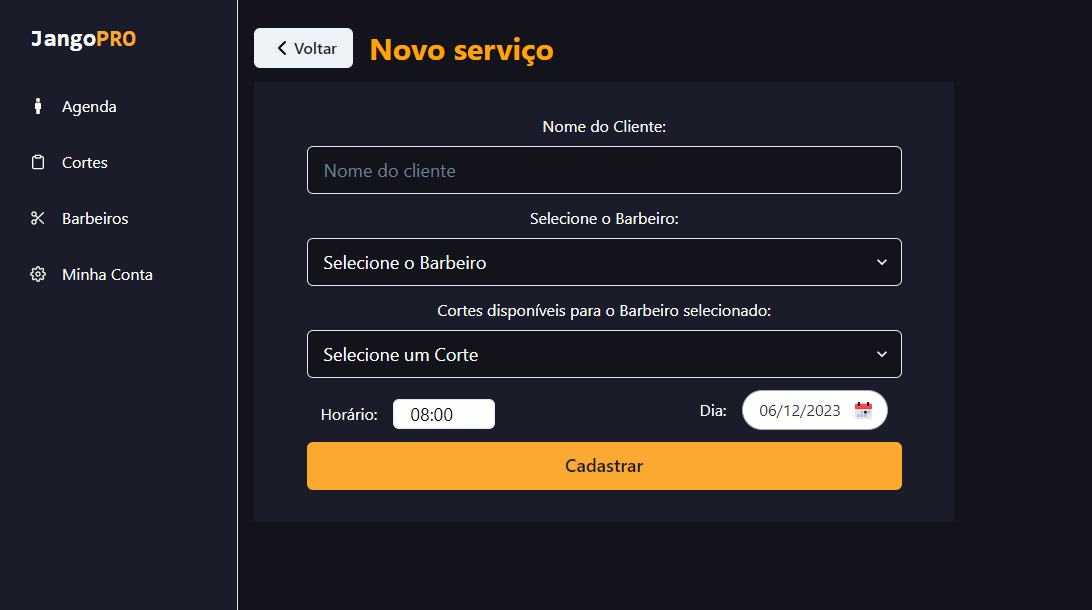
\includegraphics[width=.3\textwidth]{imgs/Agendamento.png}
    \caption{Agendamento}
    \label{fig:agendamento}
\end{figure}
\begin{figure}[!ht]
    \centering
    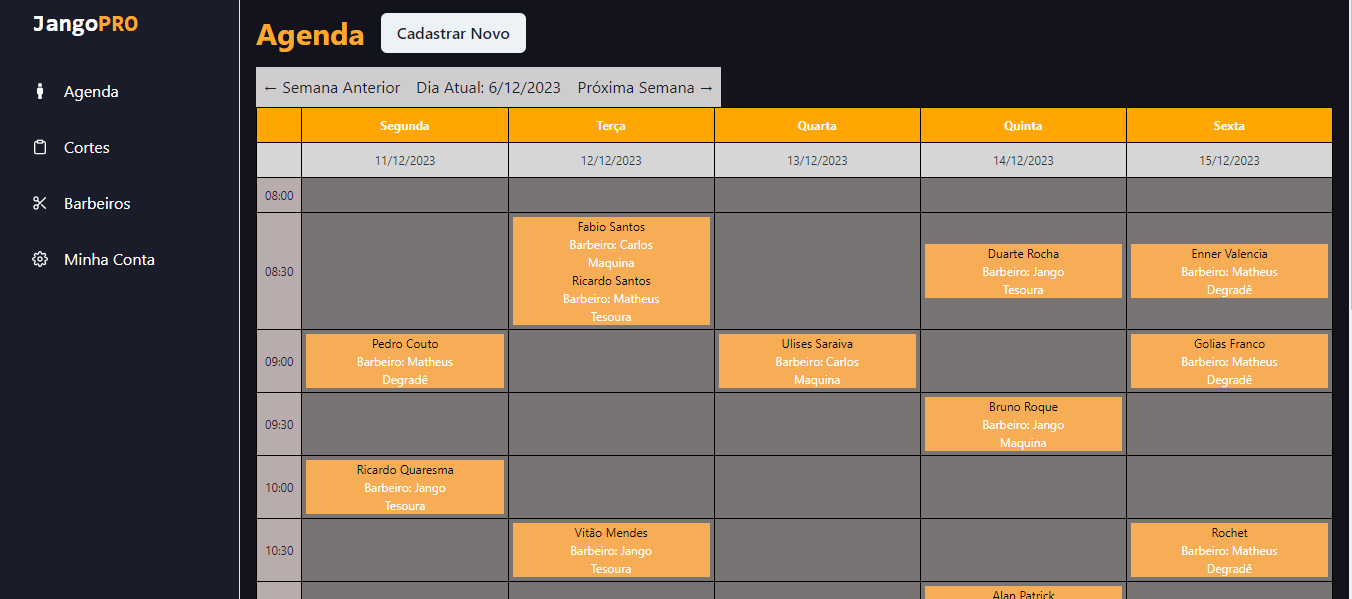
\includegraphics[width=.3\textwidth]{imgs/Dashboard.png}
    \caption{Dashboard}
    \label{fig:dashboard}
\end{figure}
\begin{figure}[!ht]
    \centering
    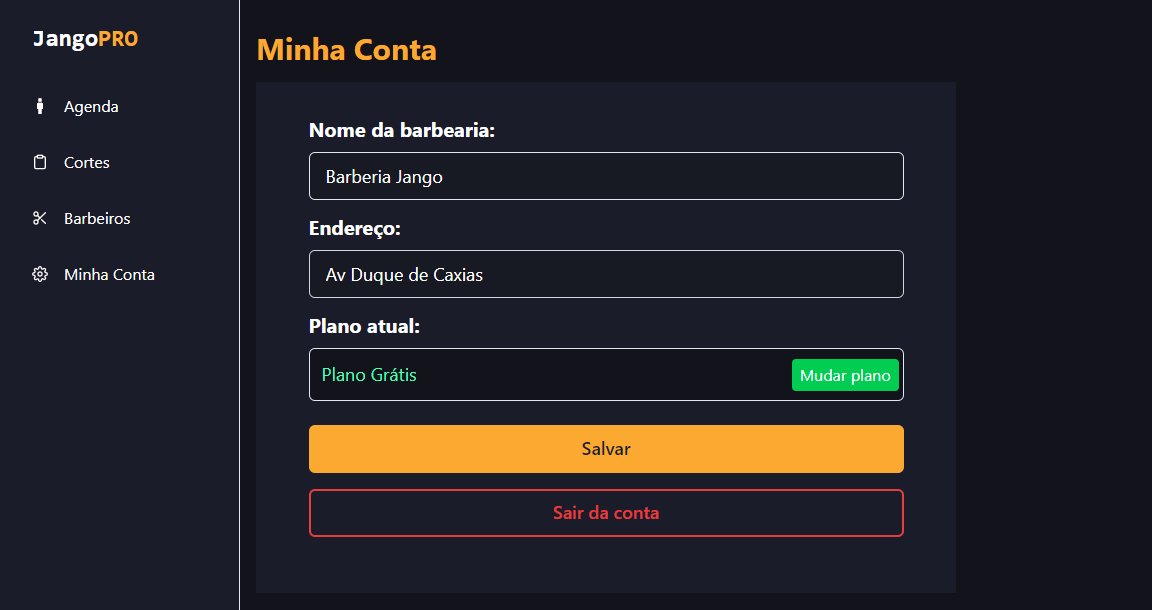
\includegraphics[width=.3\textwidth]{imgs/conta.png}
    \caption{Conta}
    \label{fig:conta}
\end{figure}

\section{Considerações Finais}

No desenvolvimento do sistema JangoPRO, foi possível alcançar diversos objetivos específicos que foram estabelecidos desde o início do projeto. Ao analisar as funcionalidades implementadas e os diferenciais apresentados, é possível destacar as seguintes conclusões:

\subsection{Alcance dos Objetivos:}

1. \textbf{Integração Completa:}
   - A proposta de integração completa, abrangendo desde o cadastro da barbearia até o agendamento personalizado, foi totalmente atendida. O JangoPRO oferece uma solução holística que simplifica a administração e otimiza a experiência do cliente.

2. \textbf{Personalização e Flexibilidade:}
   - A capacidade de personalização, tanto no cadastro de cortes quanto na escolha de planos, demonstra a flexibilidade do sistema em se adaptar às necessidades específicas de cada barbearia. A abordagem modular do JangoPRO proporciona uma gestão personalizada.

3. \textbf{Eficiência Operacional e Experiência do Cliente:}
   - A ênfase na eficiência operacional, evidenciada pelo controle detalhado de agendamentos, reflete diretamente na melhoria da experiência do cliente. A minimização do tempo de espera e a notificação automática contribuem para uma interação mais ágil e positiva.

\subsection{Reflexão sobre os Diferenciais:}

Ao comparar o JangoPRO com sistemas relacionados, fica claro que os diferenciais propostos, como a integração holística, personalização avançada e foco na experiência do cliente, foram efetivamente alcançados. Esses aspectos não apenas atendem às demandas operacionais identificadas, mas também elevam o sistema a um patamar de excelência na gestão de barbearias.

\subsection{Perspectivas Futuras:}

Como todo projeto dinâmico, o JangoPRO está aberto a evoluções futuras. Possíveis melhorias incluem a implementação de análises de desempenho, expansão de funcionalidades de fidelidade do cliente e integração com plataformas de pagamento digital.

Em conclusão, o JangoPRO emerge como uma solução eficaz e inovadora para a gestão de barbearias, cumprindo os objetivos estabelecidos e estabelecendo novos padrões de eficiência e personalização no setor. O desenvolvimento contínuo e a adaptação às necessidades do mercado são fundamentais para assegurar que o JangoPRO permaneça na vanguarda das soluções tecnológicas para barbearias.


\subsection{Dificuldades Encontradas}

Durante a execução do projeto JangoPRO, diversas dificuldades foram enfrentadas, proporcionando aprendizados valiosos que podem contribuir para futuros trabalhos relacionados. As principais dificuldades identificadas incluem:

\subsection{Integração de Tecnologias:}

A integração de múltiplas tecnologias, como Prisma, Node.js, e Next.js, apresentou desafios iniciais, especialmente no que diz respeito à configuração e sincronização entre essas ferramentas. A necessidade de lidar com diferentes ambientes e dependências demandou um tempo significativo para compreensão e resolução de conflitos.

\subsection{Validação de Dados:}

A implementação da validação de dados, em especial no que se refere aos requisitos de senha e e-mail, exigiu uma abordagem cuidadosa. Encontrar um equilíbrio entre garantir a segurança dos dados e proporcionar uma experiência de usuário fluida foi um desafio relevante.

\subsection{Testes de Usabilidade:}

A realização de testes de usabilidade eficazes, que permitissem identificar possíveis pontos de atrito na interação do usuário com o sistema, foi uma etapa desafiadora. A diversidade de perfis de usuários e a garantia de uma experiência intuitiva exigiram iterações frequentes.

\subsection{Documentação Abrangente:}

A elaboração de uma documentação abrangente, que contemplasse desde o código-fonte até as instruções de uso, mostrou-se como uma tarefa complexa. Manter a documentação atualizada à medida que o sistema evoluía demandou uma gestão cuidadosa do tempo.

\subsection{Adaptação às Mudanças de Requisitos:}

Mudanças nos requisitos durante o desenvolvimento, embora inevitáveis, representaram desafios no ajuste de funcionalidades já implementadas. A flexibilidade para se adaptar a novas demandas sem comprometer a estabilidade do sistema exigiu uma abordagem iterativa.

Essas dificuldades encontradas servem como lições valiosas para projetos futuros. A transparência em reconhecer e enfrentar desafios contribui não apenas para o aprimoramento do projeto em questão, mas também para o desenvolvimento contínuo das habilidades e boas práticas em projetos subsequentes.

\end{document}